\chapter{Results}\label{ch:results}

\section{Writing events one by one}

\subsection{Total events written}
Figure \ref{fig:total-individual-events-written} shows how many events were written to each lakehouse table. We can see that the first run of each SUT performed slightly better, before stabilizing at lower levels in the subsequent warm runs. Therefore, we focus on results from warm runs throughout the rest of this thesis. Other results can be found in Appendix \ref{ch:additional-results}.

\begin{figure}[h!]
	\centering
	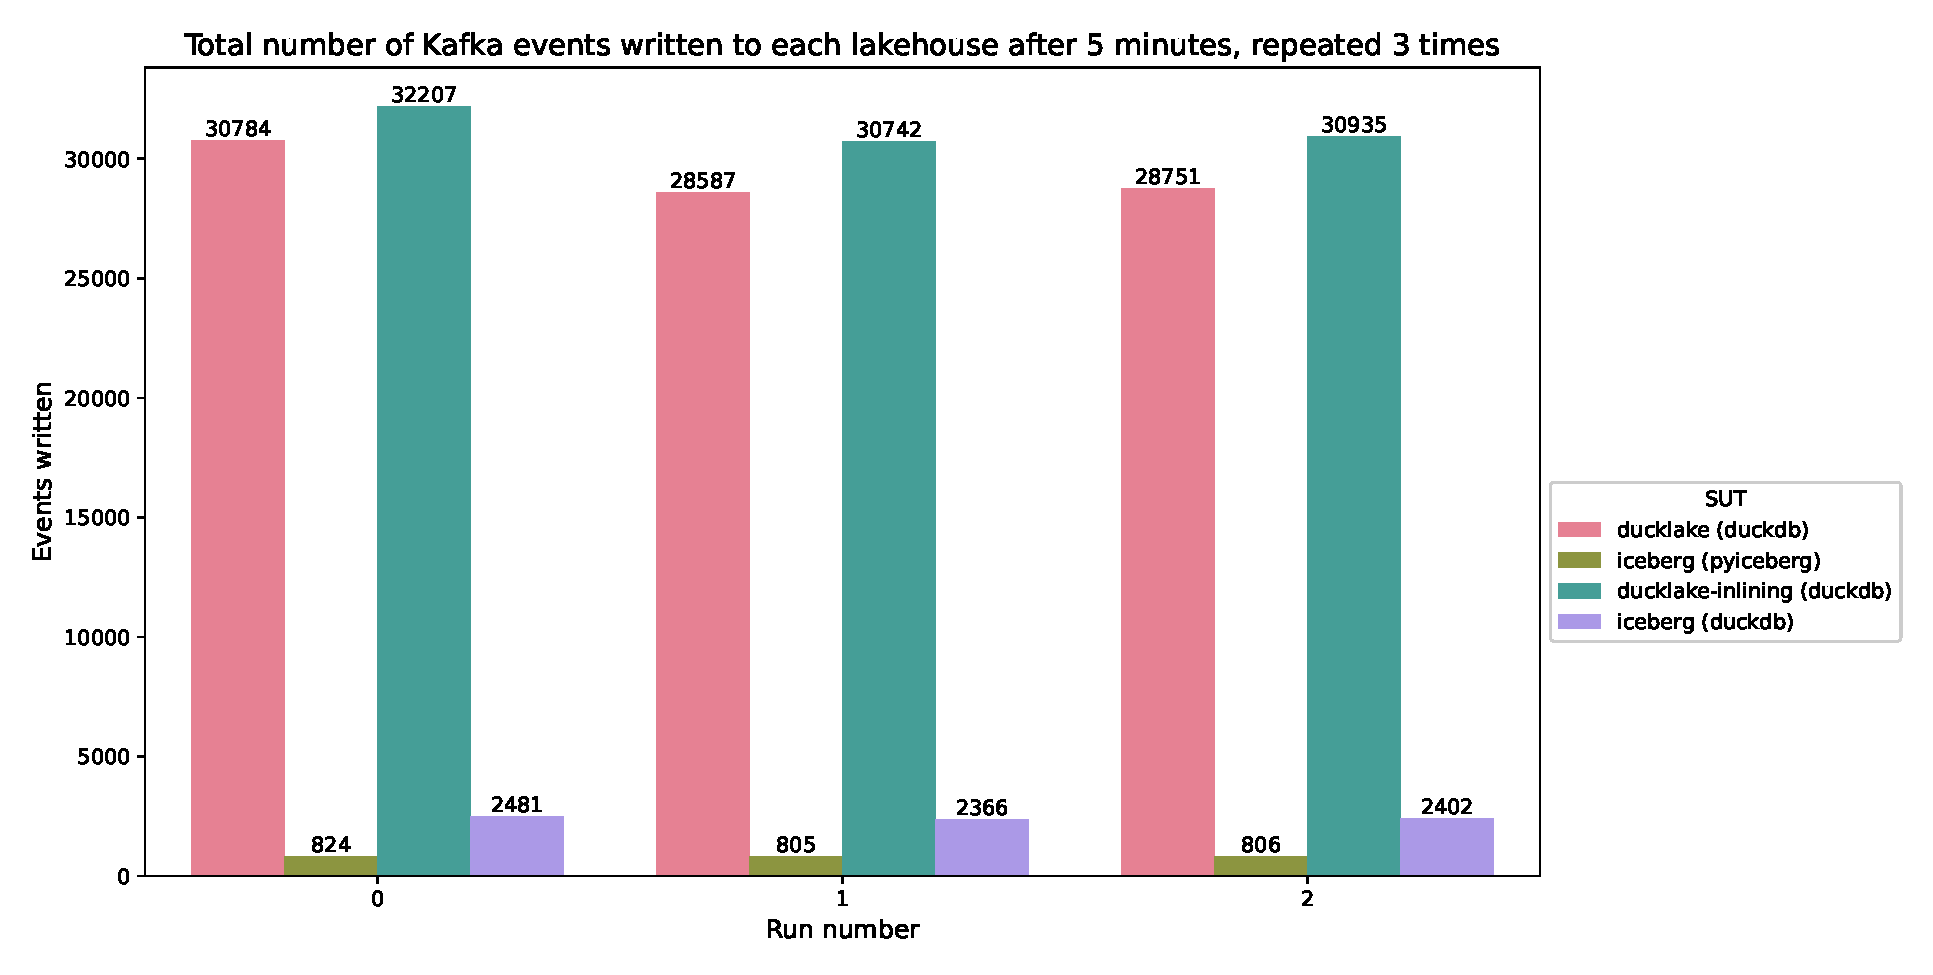
\includegraphics[width=\linewidth]{imgs/total-individual-events-written.eps}
	\caption{Number of events written one by one to each SUT in a time span of 5 minutes. The run numbers correspond to the repetitions of each experiment, where run 0 is considered cold and runs 1 and 2 are considered warm.}
	\label{fig:total-individual-events-written}
\end{figure}

Looking at the amount of events written to the different SUTs in Figure \ref{fig:total-individual-events-written}, we can see that DuckLake had a much higher throughput than Iceberg. Using DuckDB did improve Iceberg's throughput, but it was nonetheless much lower than DuckLake's.

\begin{figure}[h!]
	\centering
	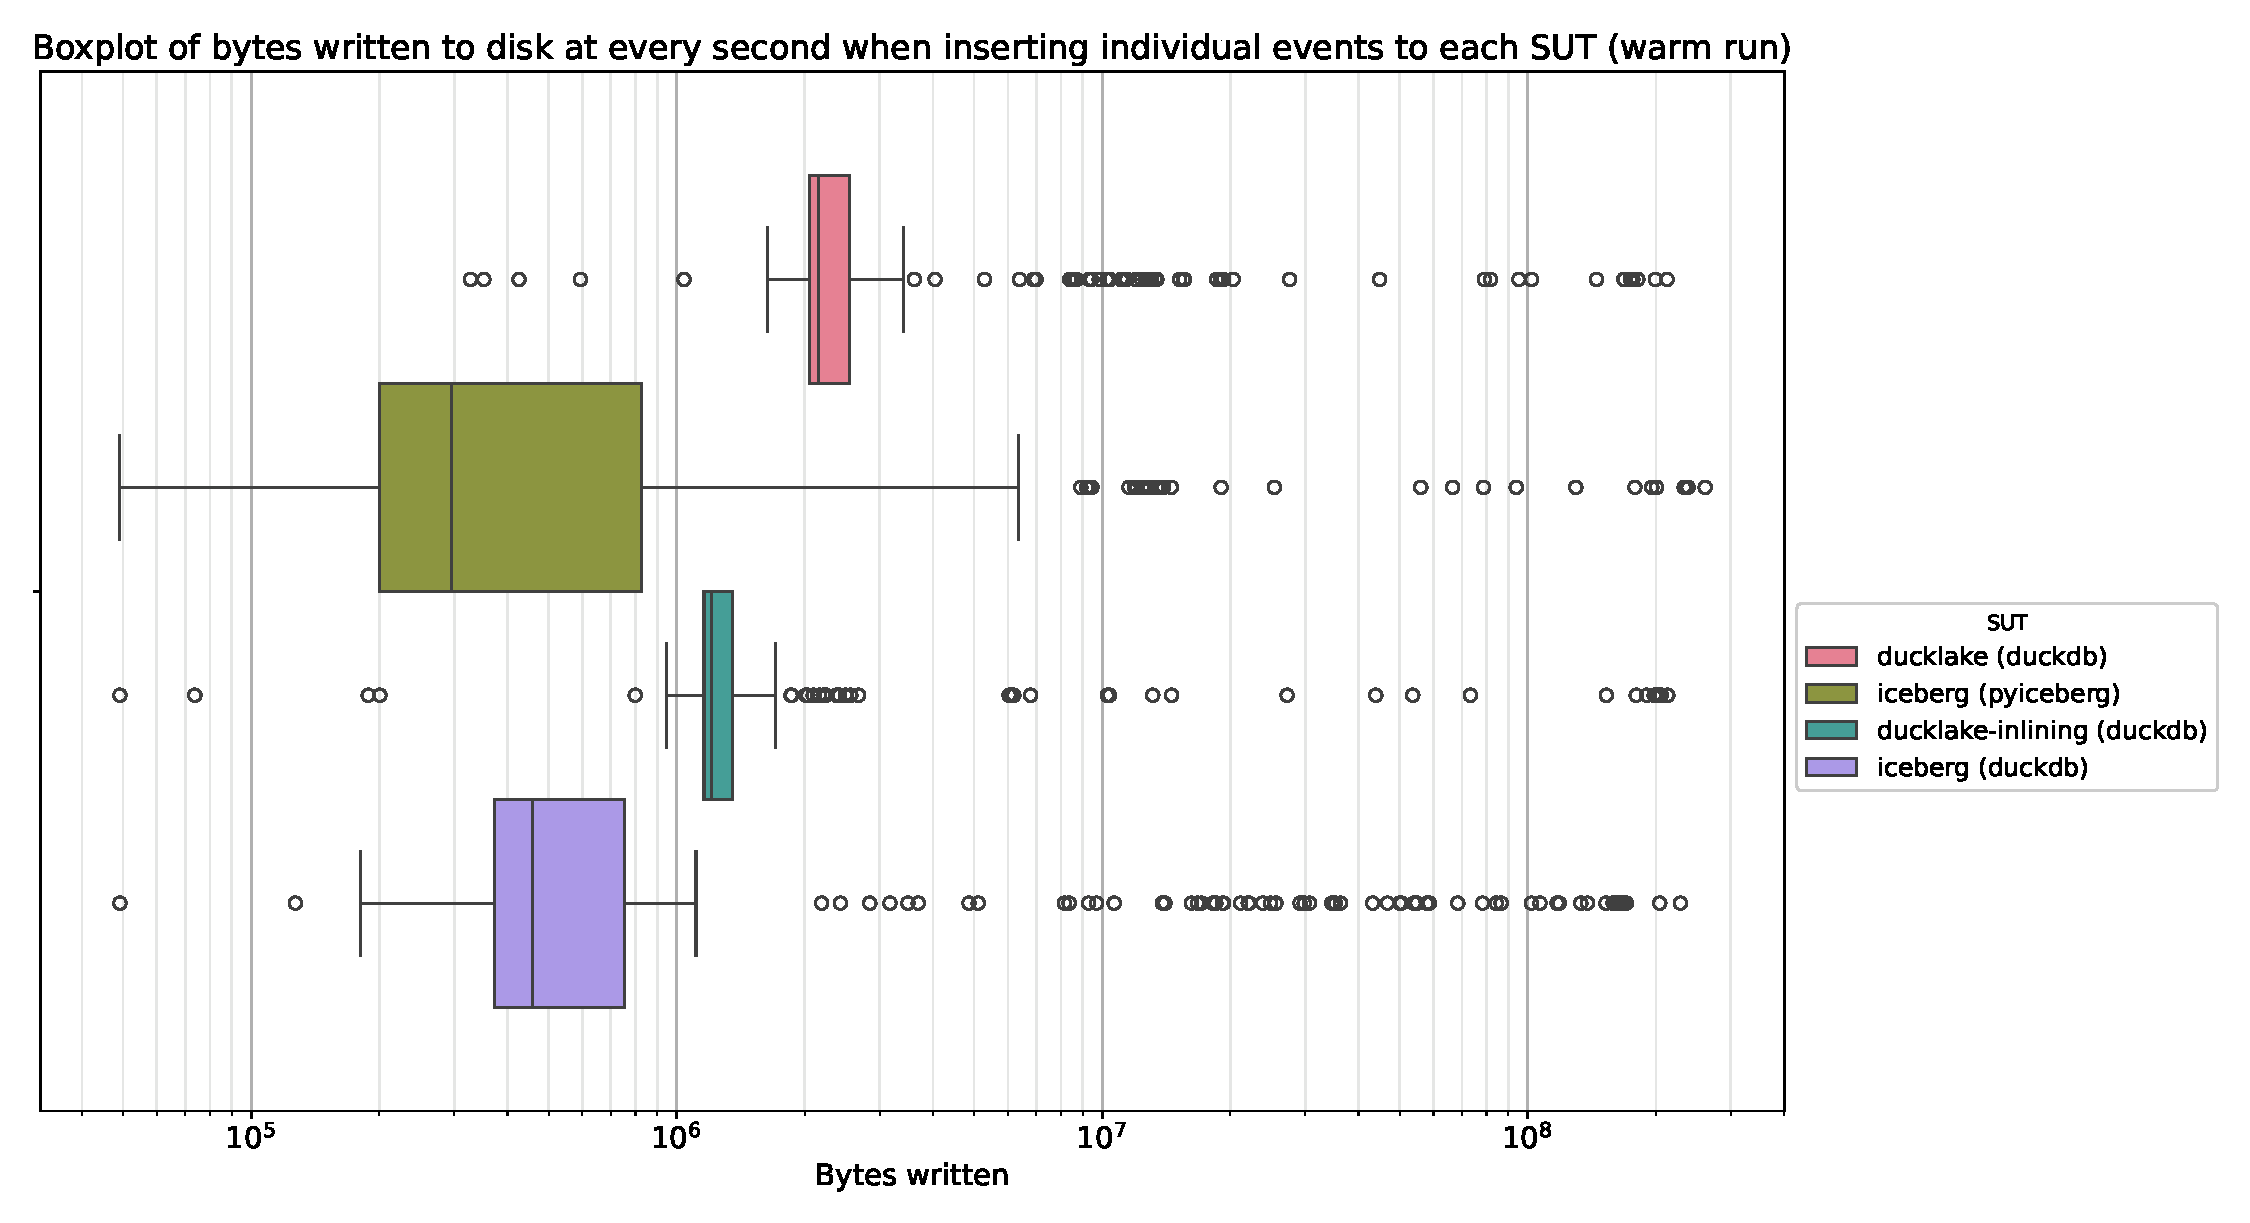
\includegraphics[width=\linewidth]{imgs/box-bytes-written-individual.eps}
	\caption{Boxplot of bytes written to disk at every second when inserting individual events to each SUT (warm run). The measurements were taken at intervals of 1 second.}
	\label{fig:box-bytes-written-individual}
\end{figure}

\begin{table}[h!]
	\centering
	\begin{tabular}{|c|c|c|}
		\hline
		\textbf{SUT} & \textbf{Median (MB)} & \textbf{IQR (MB)} \\
		\hline
		DuckLake & 2.154 & 0.502 \\
		\hline
		Iceberg (PyIceberg) & 0.291 & 0.594 \\
		\hline
		DuckLake + Inlining & 1.204 & 0.193 \\
		\hline
		Iceberg (DuckDB) & 0.459 & 0.380 \\
		\hline
	\end{tabular}
	\caption{Median and interquartile range, in megabytes, of the box plots presented in Figure \ref{fig:box-bytes-written-individual}.}
	\label{tab:median-iqr-box-bytes-individual}
\end{table}

Focusing now on the first warm run of each SUT, we see from Figure \ref{fig:box-bytes-written-individual} that DuckLake was often able to write more bytes per second than Iceberg, which is in line with the total events written, shown in Figure \ref{fig:total-individual-events-written}. We can also see from Table \ref{tab:median-iqr-box-bytes-individual} that the median number of bytes written to DuckLake was about an order of magnitude larger than that of Iceberg with PyIceberg. In addition, Iceberg + PyIceberg seems to have a more unstable rate of bytes/second, which is reflected by the highest interquartile range, i.e. spread, presented in Table \ref{tab:median-iqr-box-bytes-individual}.

\subsection{Write times}
Looking at Figure \ref{fig:box-write-times-individual}, we can see that DuckLake has more consistent write times than Iceberg + PyIceberg, based on the difference in the spread between them. Using Iceberg with DuckDB produces a smaller spread, and thus more consistent write times, but its median is still around an order of magnitude slower than both DuckLake runs. The median write times of each SUT are consistent with their respective amount of bytes/second and events written (Figures \ref{fig:box-bytes-written-individual} and \ref{fig:total-individual-events-written}).

\begin{figure}[h!]
	\centering
	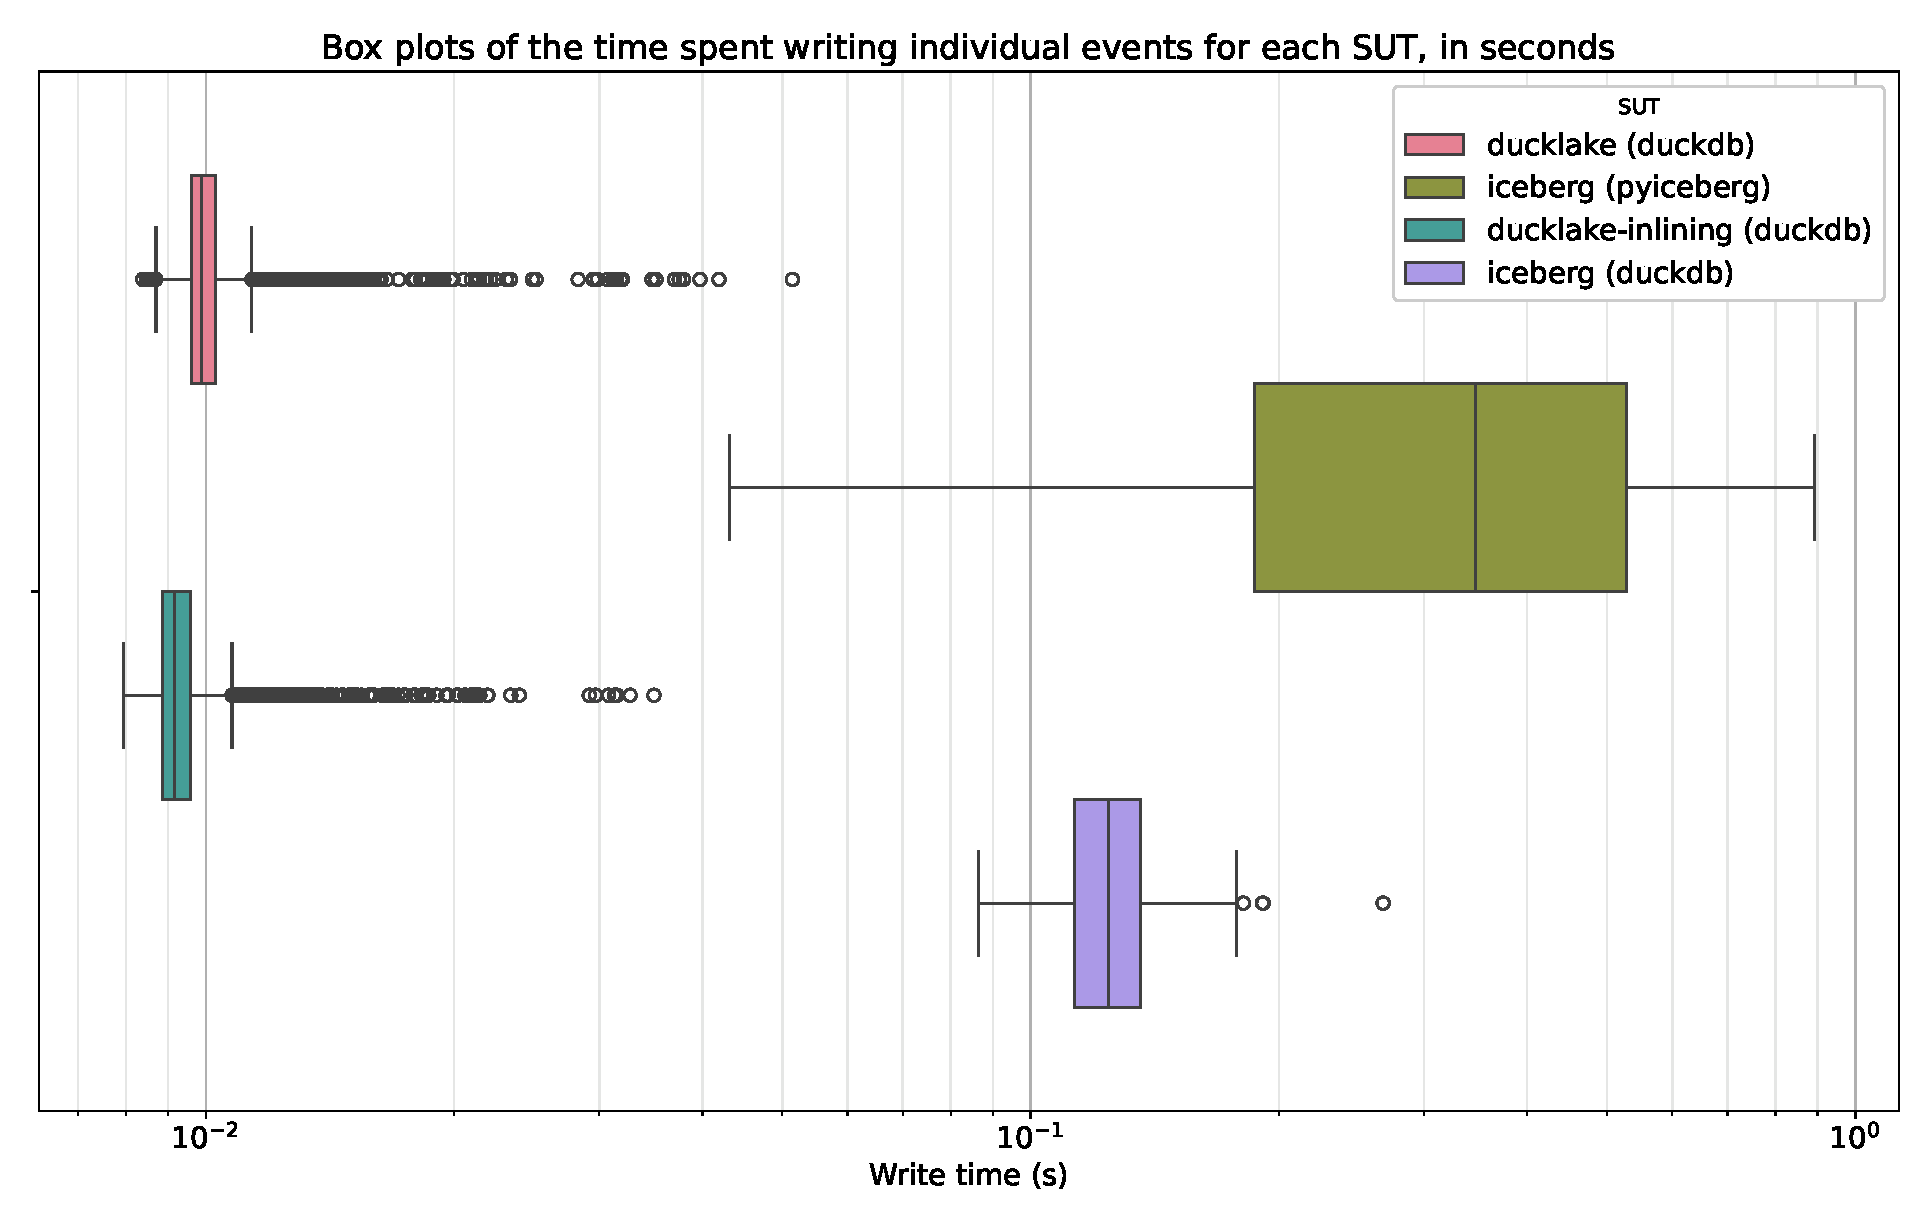
\includegraphics[width=\linewidth]{imgs/box-write-times-individual.eps}
	\caption{Box plots of the time spent writing each individual event to the lakehouse tables during the first warm run, in seconds.}
	\label{fig:box-write-times-individual}
\end{figure}

\begin{table}[h!]
	\centering
	\begin{tabular}{|c|c|c|}
		\hline
		\textbf{SUT} & \textbf{Median (ms)} & \textbf{IQR (ms)} \\
		\hline
		DuckLake & 9.889 & 0.667 \\
		\hline
		Iceberg (PyIceberg) & 346.208 & 341.194 \\
		\hline
		DuckLake + Inlining & 9.169 & 0.711 \\
		\hline
		Iceberg (DuckDB) & 124.303 & 22.650 \\
		\hline
	\end{tabular}
	\caption{Median and interquartile range, in milliseconds, of the box plots presented in Figure \ref{fig:box-write-times-individual}.}
	\label{tab:median-iqr-box-write-times-individual}
\end{table}

We observed that the write times for Iceberg increase over time, as shown in Figure \ref{fig:scatter-write-times-over-time-individual}, which explains the larger spread in the data when compared to other SUTs. Although using Iceberg with DuckDB help control the spread of write times, we can see from Figure \ref{fig:scatter-write-times-over-time-individual} that they still get larger, as more data is written. By contrast, DuckLake's write times seems to stay more or less constant throughout the whole run.

\begin{figure}[h!]
	\centering
	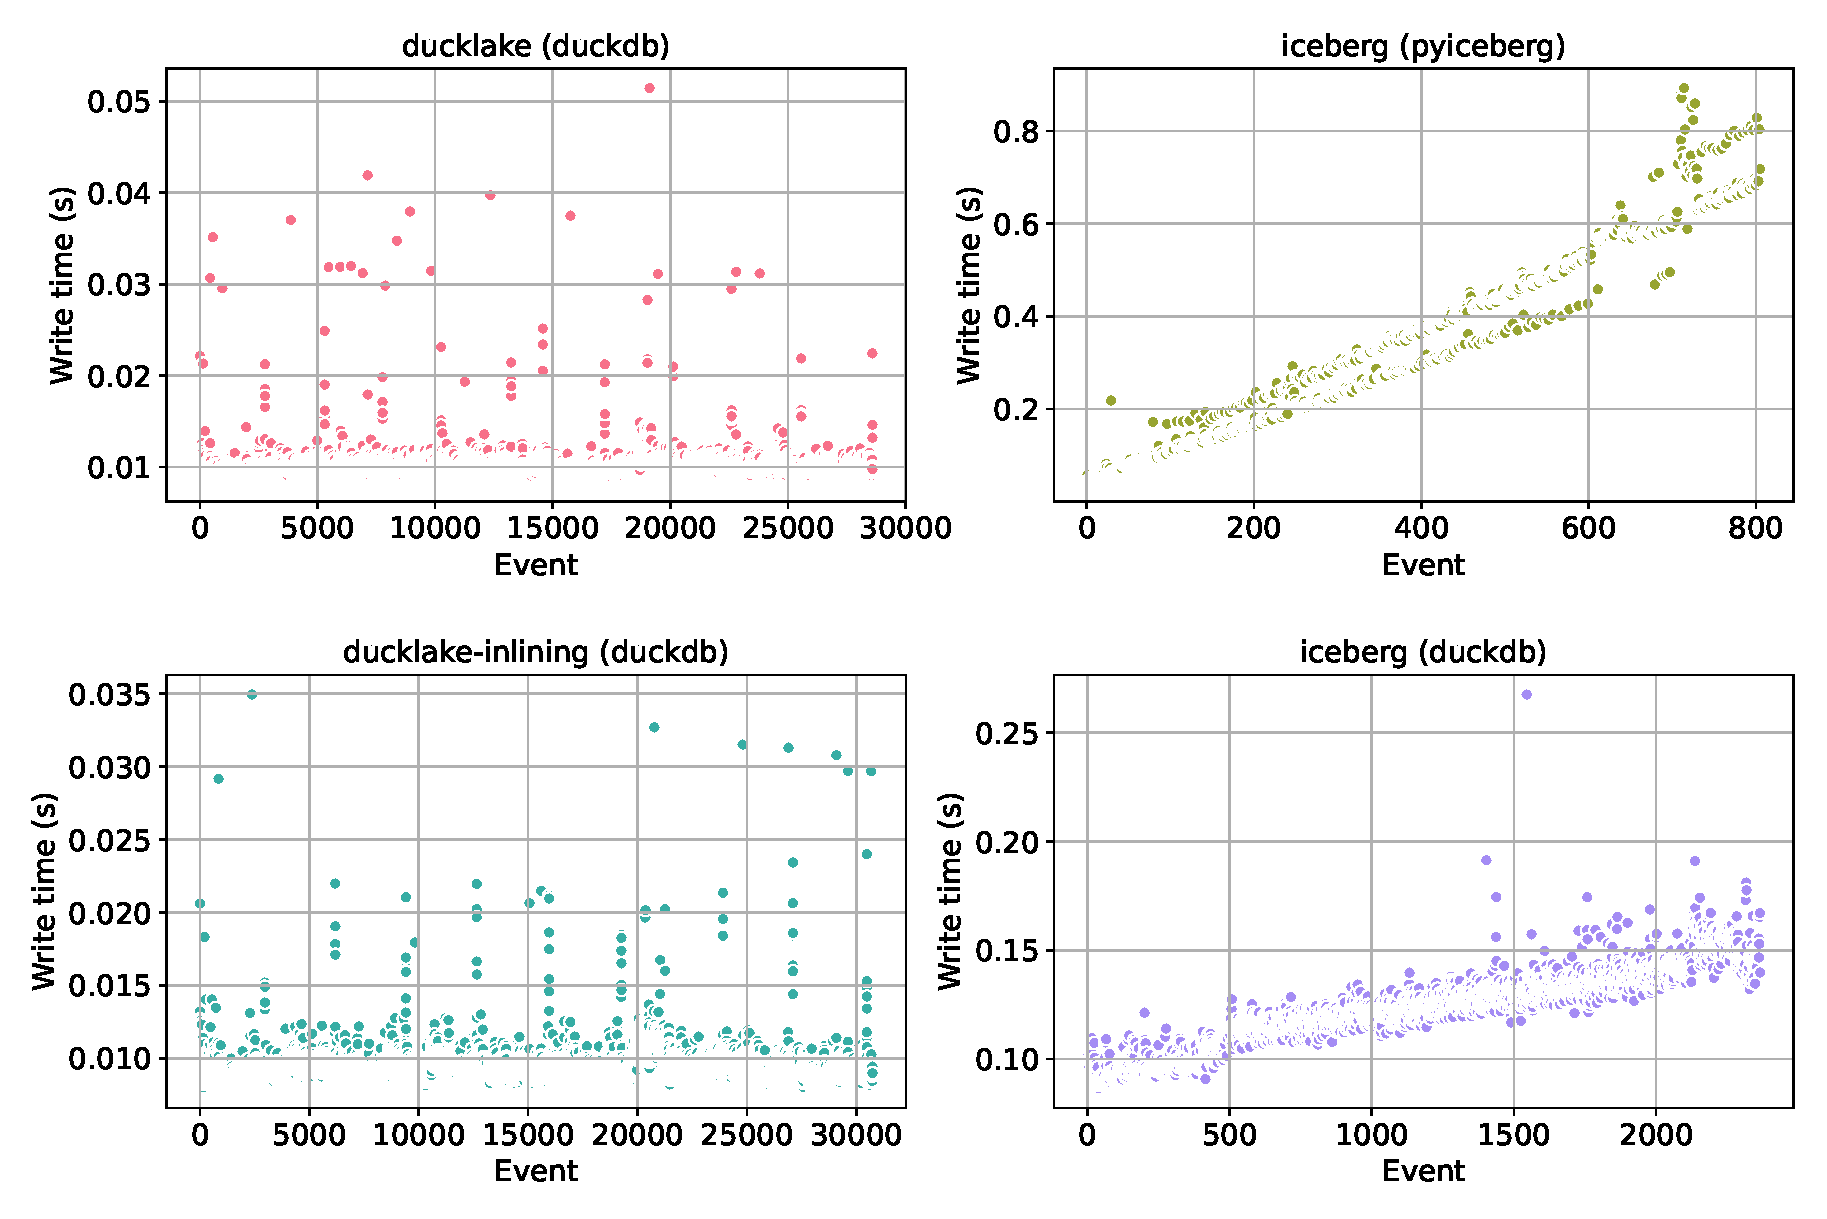
\includegraphics[width=\linewidth]{imgs/scatter-write-times-over-time-individual.eps}
	\caption{Scatter plot of time spent writing individual event to the lakehouse tables during the first warm run, in seconds.}
	\label{fig:scatter-write-times-over-time-individual}
\end{figure}


\begin{table}[h!]
	\centering
	\begin{tabular}{|c|c|}
		\hline
		\textbf{Run number} & \textbf{Flush time (ms)} \\
		\hline
		0 & 219.874 \\
		\hline
		1 & 205.867 \\
		\hline
		2 & 193.615 \\
		\hline
	\end{tabular}
	\caption{Time taken by each DuckLake + Inlining run to flush inlined data to a single Parquet file, in milliseconds.}
	\label{tab:times-flush-inlined-individual}
\end{table}

Regarding the DuckLake instance with inlining enabled, we find that the time taken to flush the inlined events to a Parquet file on disk was around 200 milliseconds, as shown in Table \ref{tab:times-flush-inlined-individual}. This is about $20\times$ slower than the median write time of DuckLake without inlining, and about $2\times$ slower than the median of Iceberg with DuckDB. However, DuckLake with inlining enabled was able to outperform the median write time of Iceberg with PyIceberg by around $1.5\times$.

\subsection{Read times}

\begin{figure}[h!]
	\centering
	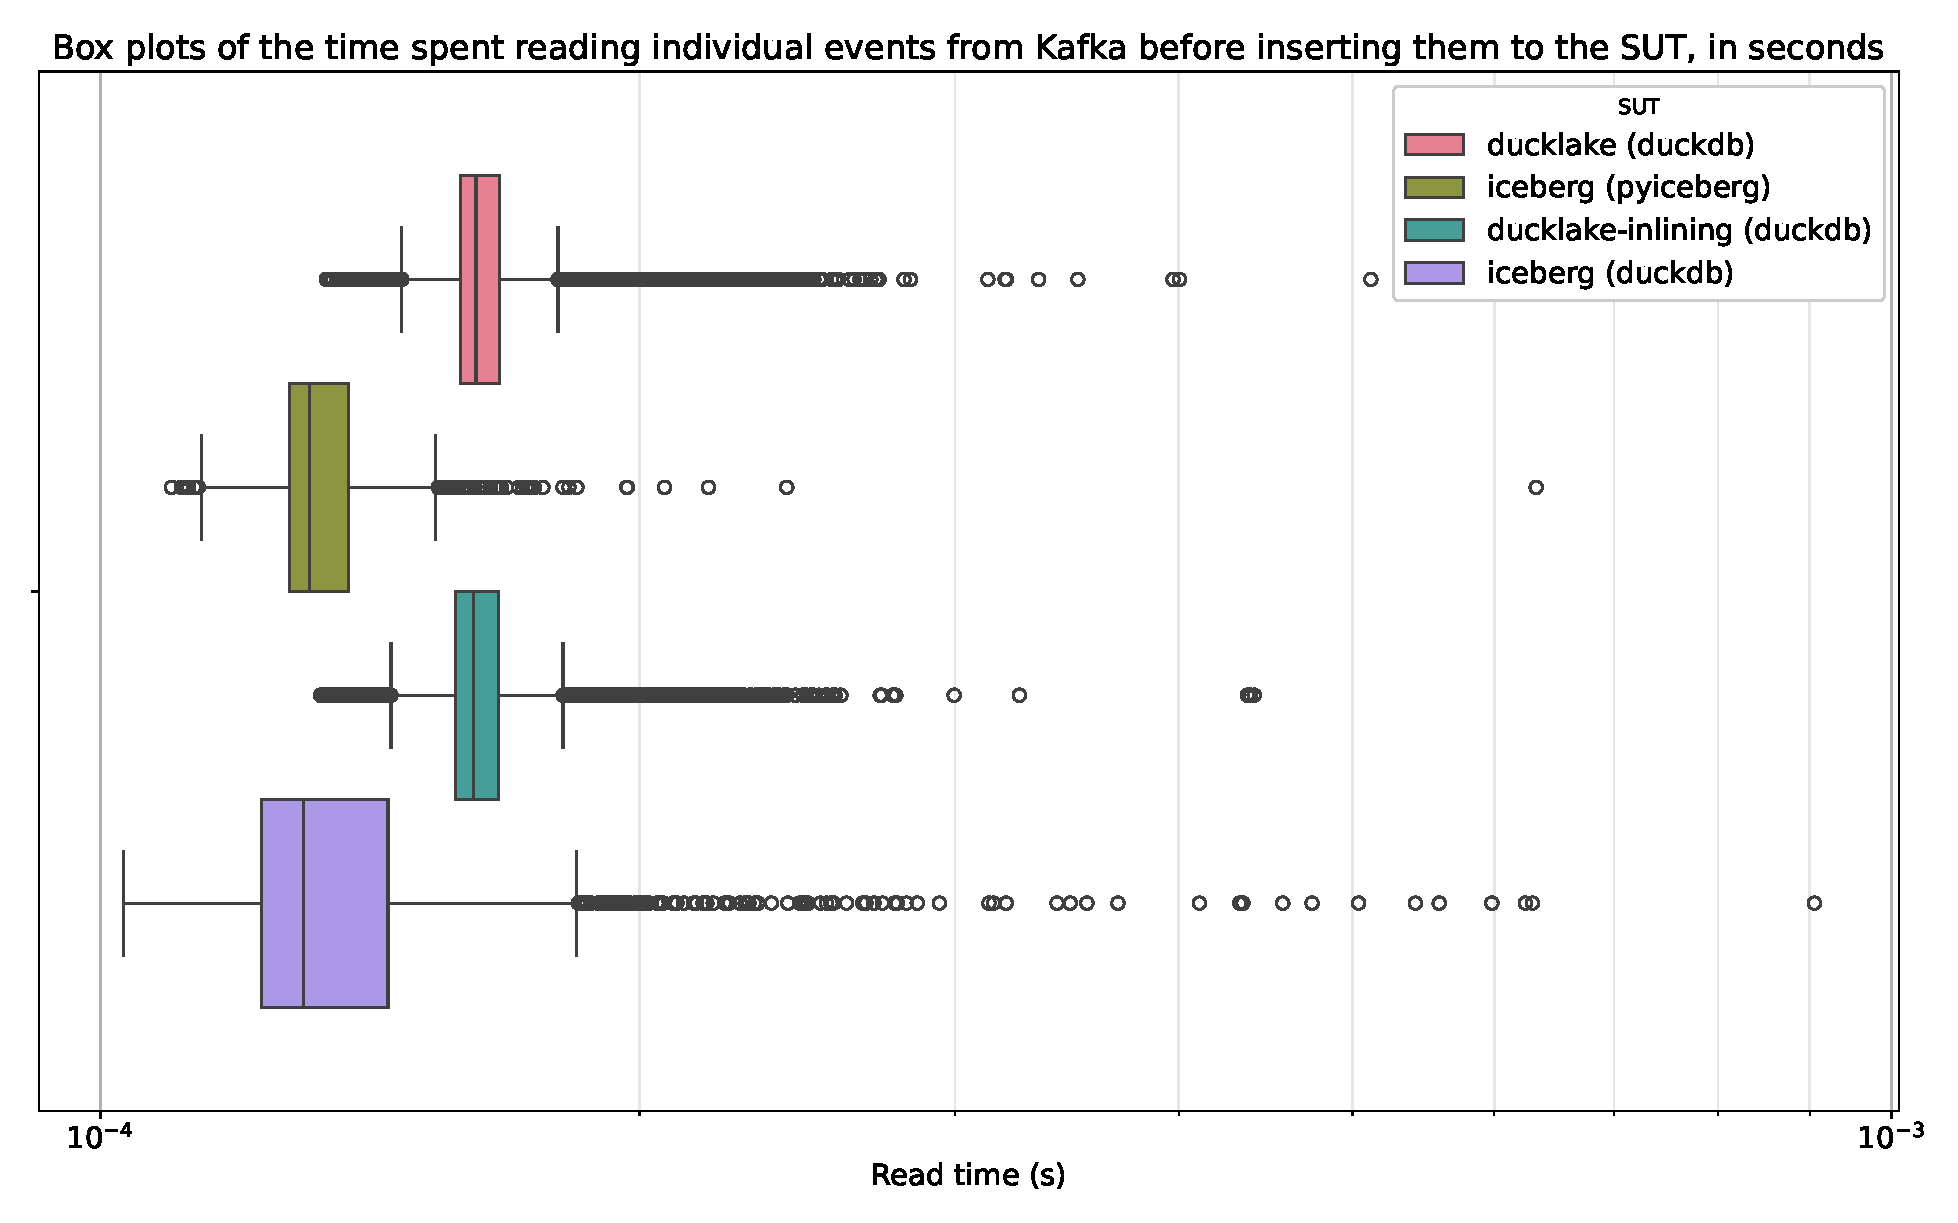
\includegraphics[width=\linewidth]{imgs/box-read-times-individual.eps}
	\caption{Box plots of the time spent reading individual events from Kafka during the first warm run of each SUT, in seconds.}
	\label{fig:box-read-times-individual}
\end{figure}

The box plots in Figure \ref{fig:box-read-times-individual} go over the time spent reading each individual event from the Kafka broker. We can see that the median read times of DuckLake runs were slightly higher than Iceberg's, but the almost all read times were lower than 1 millisecond, with most times staying between 0.1 and 0.2 milliseconds. These measurements indicate that no system had a major advantage over others due to significantly higher read times.

\subsection{CPU usage}
We observed that Iceberg with DuckDB consistently utilized a higher percentage of the CPU than the other three SUTs. Nonetheless, all systems were mostly stable throughout the runs, except for a few spikes and dips, as shown in Figure \ref{fig:cpu-usage-individual-events}. These observations can be attributed to the noise caused by other processes running in the background, such as the Docker containers or even OS processes.

\begin{figure}[h!]
	\centering
	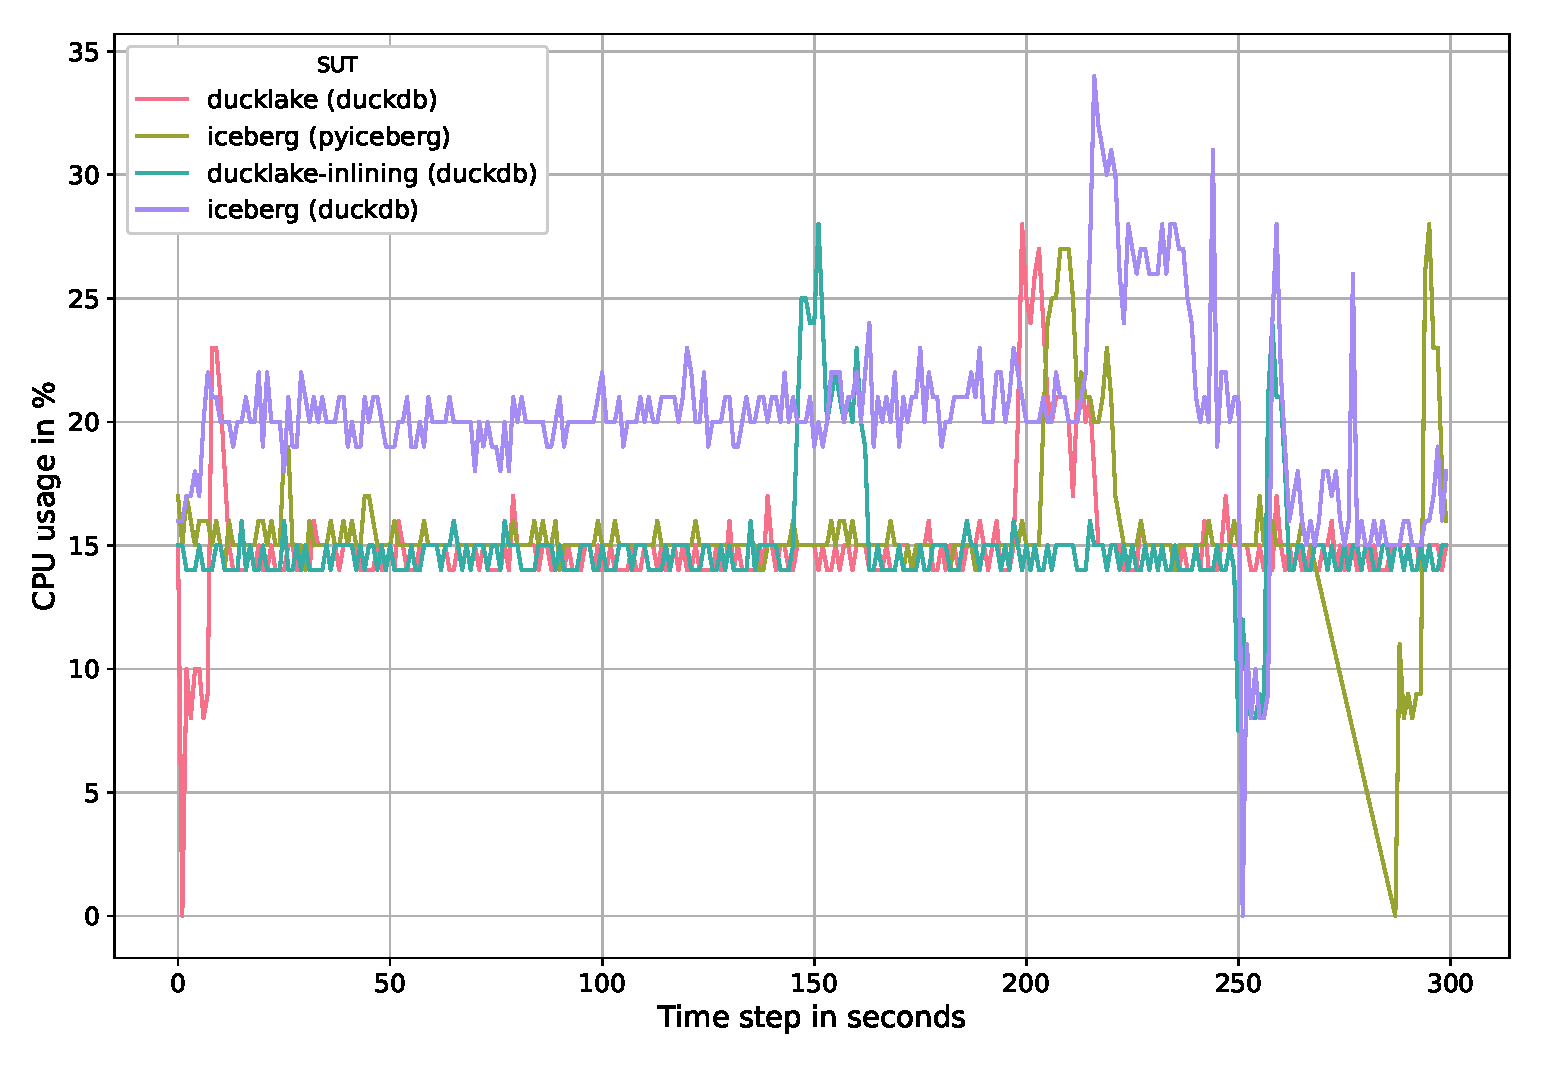
\includegraphics[width=\linewidth]{imgs/cpu-usage-individual-events.eps}
	\caption{CPU usage percentage measured at every second throughout each run of writing individual events to SUTs.}
	\label{fig:cpu-usage-individual-events}
\end{figure}

\section{Writing events in batches of 1,000}

\subsection{Total events written}
Figure \ref{fig:total-batched-events-written} shows the total number of events written to each SUT when writing data in batches of 1,000 events. As observed in the previous experiments, the cold run was slightly better than the warm runs, so we focus on the latter instead.

We can see that all systems performed significantly better than when events were written one by one to the lakehouse tables. The biggest improvement can be noticed when using Iceberg with DuckDB, which managed to surpass DuckLake with inlining enabled. We also observed that inlining led to a decrease of  in the amount of events written to DuckLake. That is in contrast to the previous experiments, where inlining had in fact improved the throughput of DuckLake.

\begin{figure}[h!]
	\centering
	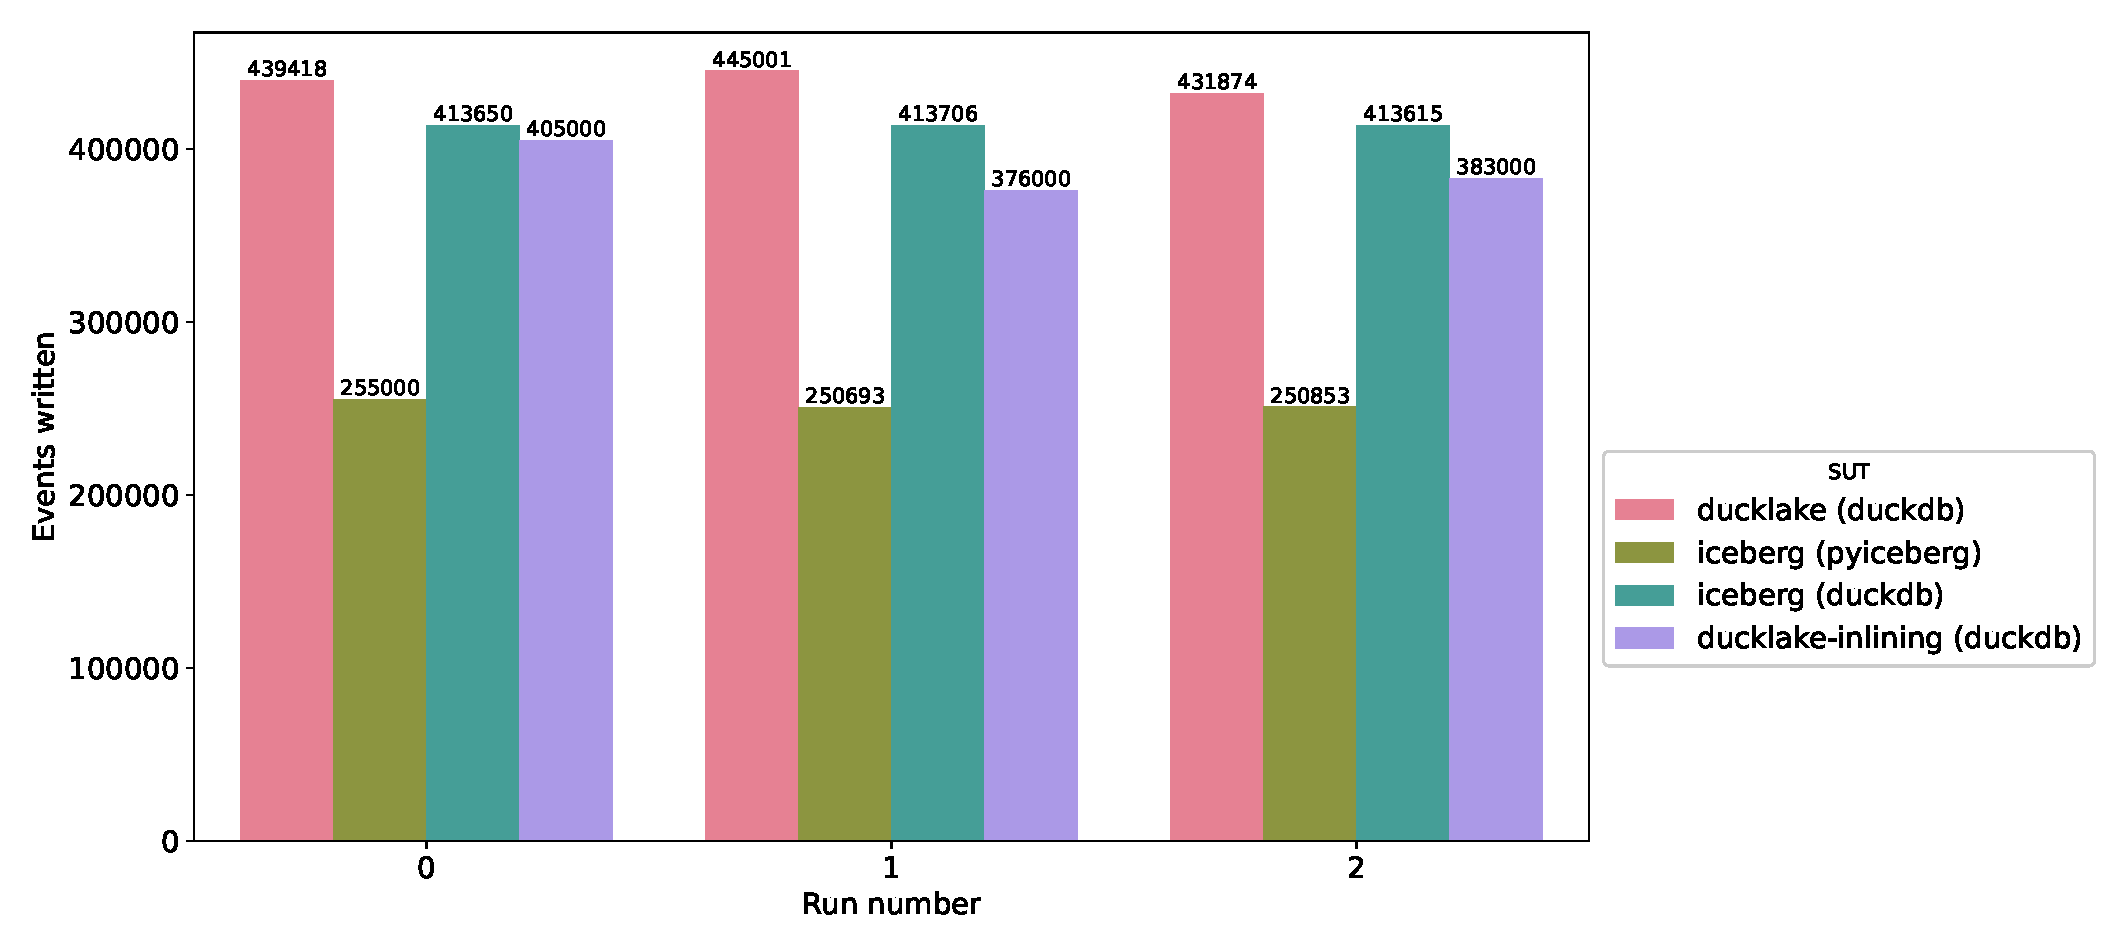
\includegraphics[width=\linewidth]{imgs/total-batched-events-written.eps}
	\caption{Number of events written in batches of 1,000 to each SUT in a time span of 5 minutes. The run numbers correspond to the repetitions of each experiment, where run 0 is considered cold and runs 1 and 2 are considered warm.}
	\label{fig:total-batched-events-written}
\end{figure}

When looking at the amount of bytes written at every second in Figure \ref{fig:box-bytes-written-batched}, we see that all systems wrote fewer bytes per second than when writing events one by one. From Table \ref{tab:median-iqr-box-bytes-batched} we can see that median number of bytes written to disk differed less between the SUTs than in the previous experiment. The exception here was DuckLake + inlining, which had a median about twice as big as the second highest median.

In terms of the spread of the data, both DuckLake instances wrote bytes at a more consistent rate than the Iceberg instances. In contrast to the previous experiment, DuckDB worsened Iceberg's data spread when compared to PyIceberg. In addition, DuckLake with inlining and Iceberg + DuckDB had less stable rates of bytes/second than their counterparts in the previous experiment. Overall, Iceberg + PyIceberg differed the least between writing individual and batched events, whereas all other three SUTs had a lower median number of bytes written per second.

\begin{figure}[h!]
	\centering
	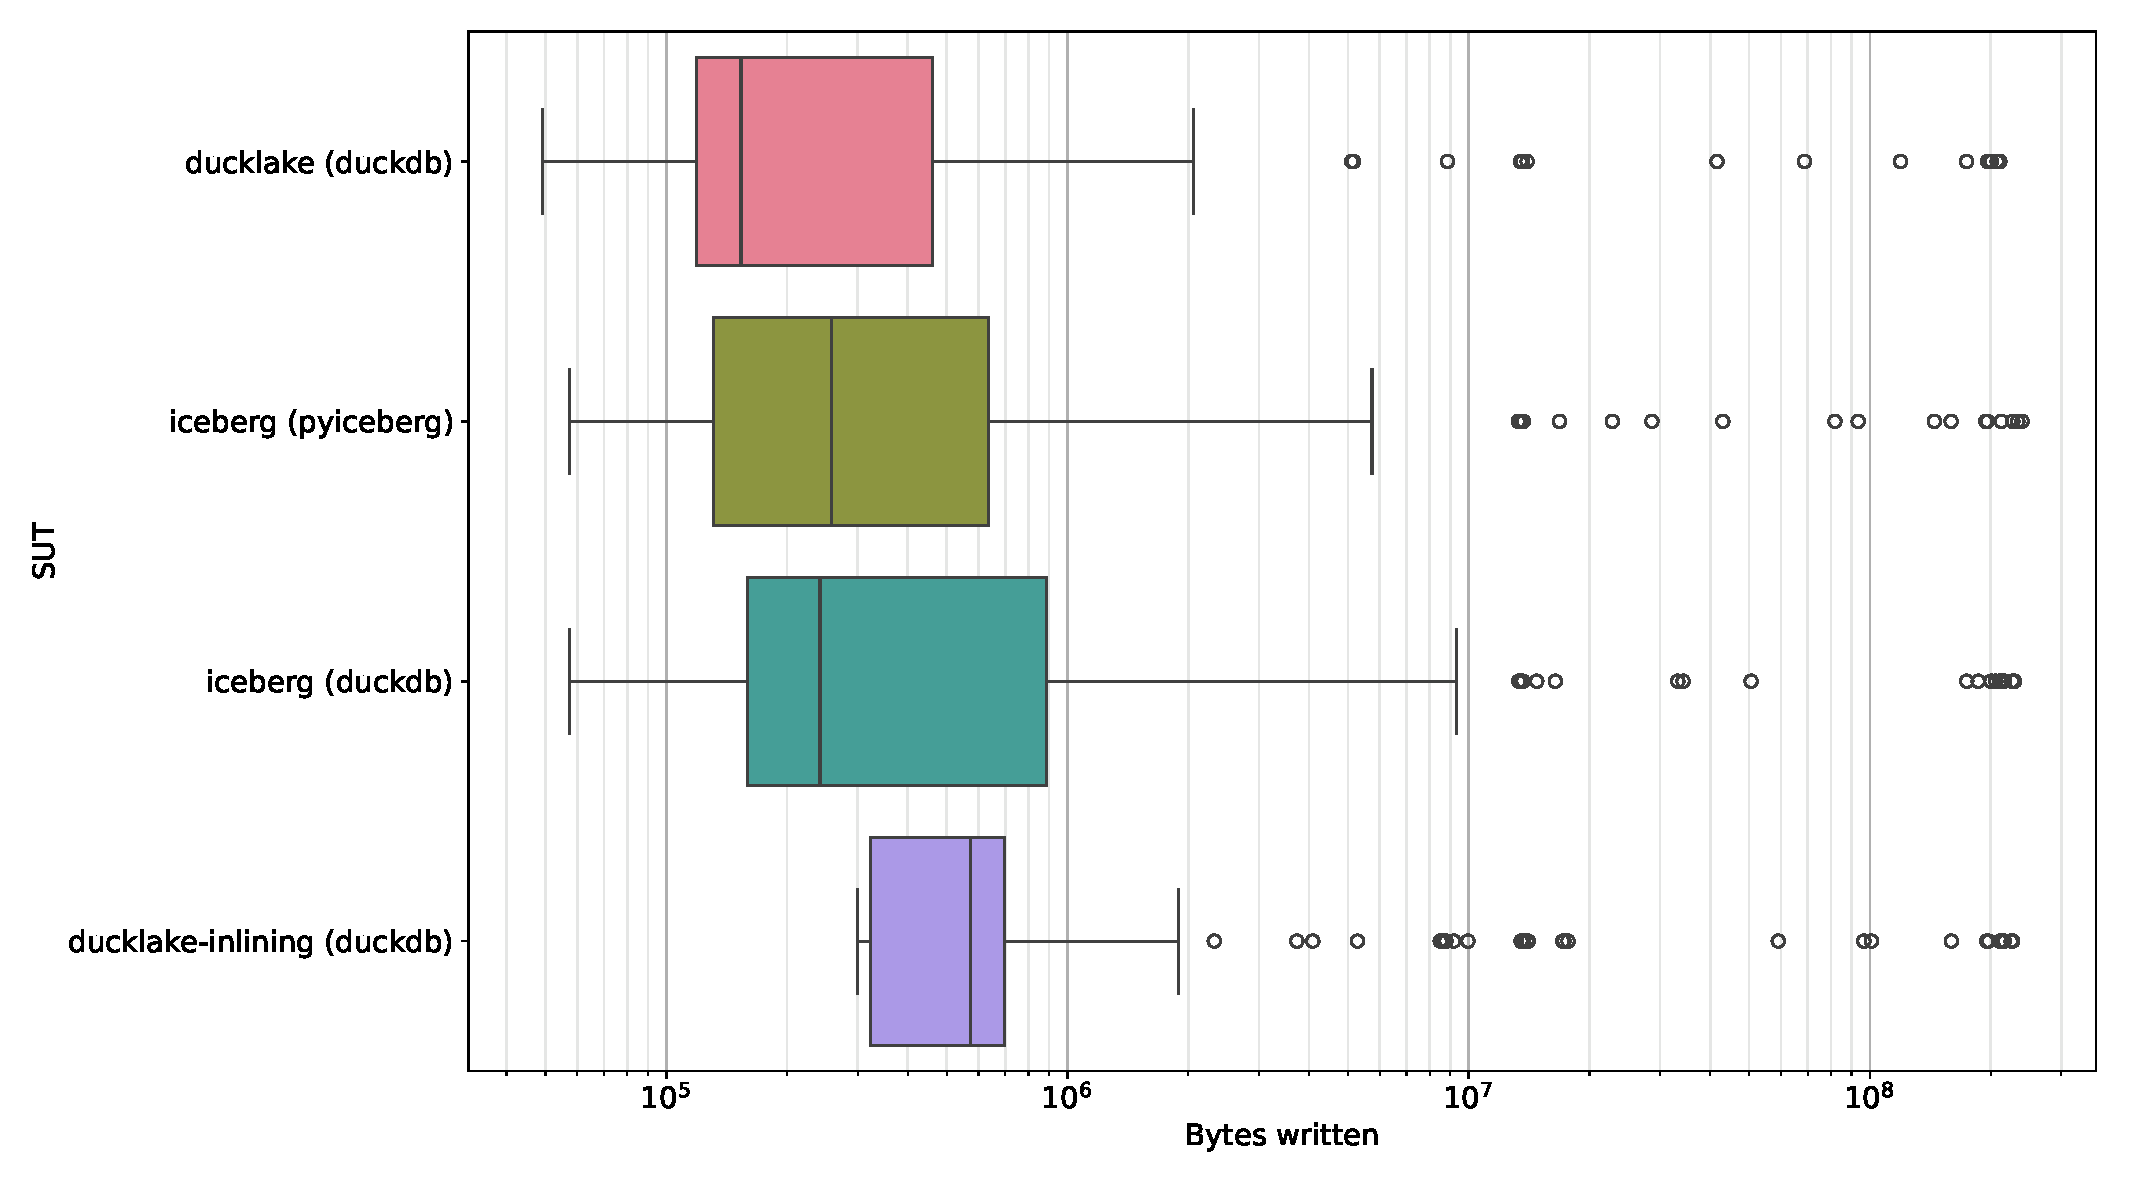
\includegraphics[width=\linewidth]{imgs/box-bytes-written-batched.eps}
	\caption{Boxplot of bytes written to disk at every second when inserting individual events to each SUT (warm run). The measurements were taken at intervals of 1 second.}
	\label{fig:box-bytes-written-batched}
\end{figure}

\begin{table}[h!]
	\centering
	\begin{tabular}{|c|c|c|}
		\hline
		\textbf{SUT} & \textbf{Median (MB)} & \textbf{IQR (MB)} \\
		\hline
		DuckLake & 0.154 & 0.341 \\
		\hline
		Iceberg (PyIceberg) & 0.258 & 0.502 \\
		\hline
		Iceberg (DuckDB) & 0.242 & 0.727 \\
		\hline
		DuckLake + Inlining & 0.573 & 0.372 \\
		\hline
	\end{tabular}
	\caption{Median and interquartile range, in megabytes, of the box plots presented in Figure \ref{fig:box-bytes-written-batched}.}
	\label{tab:median-iqr-box-bytes-batched}
\end{table}


\subsection{Write times}
The write times of the SUTs shown in Figure \ref{fig:box-write-times-batched} are in line with the results presented in Figure \ref{fig:total-batched-events-written}. We see that Iceberg + PyIceberg had the highest write times of all SUTs, with a median write time about $3\times$ higher than the second highest median (DuckLake + Inlining). For all SUTs the median write time was higher than the previous experiments because every write operation involved batches of 1,000 event, in contrast to individual events in the previous experiment.

Regarding stability of write times, Iceberg + PyIceberg was also least stable system, given by its higher IQR. All the three other systems showed a similar, lower spread in their write times.

With respect to the flush times of DuckLake + inlining, we see in Table \ref{tab:times-flush-inlined-batched} that it took around 2 seconds to flush the inlined data. This represents a tenfold increase compared to the previous experiment. Furthermore, the flush times were about $3\times$ slower than the highest median write time.

\begin{figure}[h!]
	\centering
	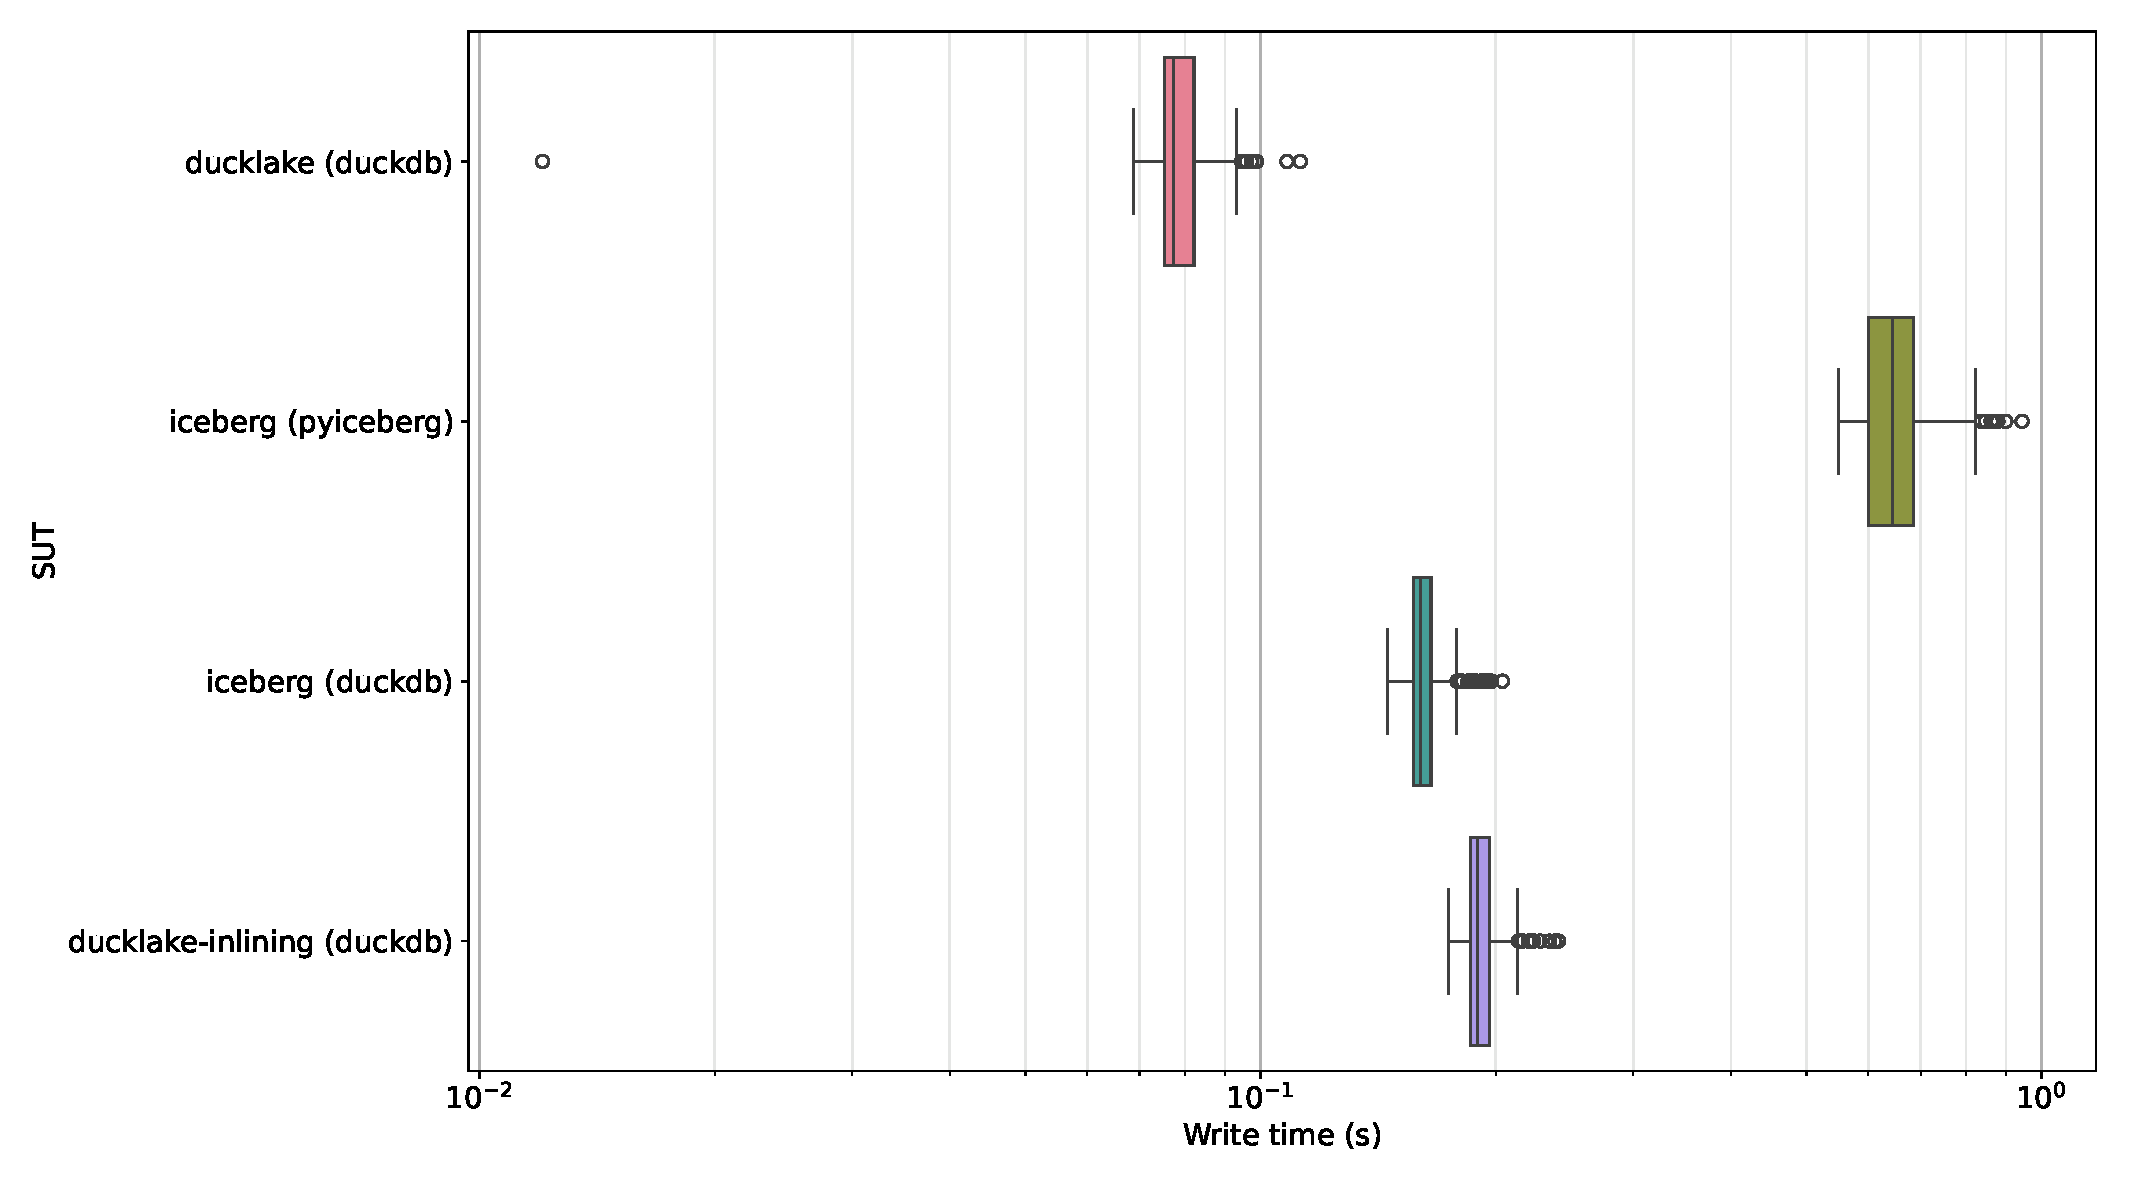
\includegraphics[width=\linewidth]{imgs/box-write-times-batched.eps}
	\caption{Box plots of the time spent writing each batch of 1,000 events to the lakehouse tables during the first warm run, in seconds.}
	\label{fig:box-write-times-batched}
\end{figure}

\begin{table}[h!]
	\centering
	\begin{tabular}{|c|c|c|}
		\hline
		\textbf{SUT} & \textbf{Median (ms)} & \textbf{IQR (ms)} \\
		\hline
		DuckLake & 77.439 & 6.942 \\
		\hline
		Iceberg (PyIceberg) & 644.842 & 84.695 \\
		\hline
		DuckLake + Inlining & 189.746 & 10.625 \\
		\hline
		Iceberg (DuckDB) & 160.086 & 8.189 \\
		\hline
	\end{tabular}
	\caption{Median and interquartile range, in milliseconds, of the box plots presented in Figure \ref{fig:box-write-times-batched}.}
	\label{tab:median-iqr-box-write-times-batched}
\end{table}

\begin{table}[h!]
	\centering
	\begin{tabular}{|c|c|}
		\hline
		\textbf{Run number} & \textbf{Flush time (s)} \\
		\hline
		0 & 2.287 \\
		\hline
		1 & 1.992 \\
		\hline
		2 & 1.974 \\
		\hline
	\end{tabular}
	\caption{Time taken by each DuckLake + inlining run to flush the inlined batches of data to a single Parquet file, in seconds.}
	\label{tab:times-flush-inlined-batched}
\end{table}

Looking now at Figure \ref{fig:scatter-write-times-over-time-batched}, we can see that write times behave in a similar way as the previous experiment. When using Iceberg with PyIceberg, we see the same effect where write times get larger as more events are added to the Iceberg table, which again explains the bigger spread of Iceberg's write times presented in Table \ref{tab:median-iqr-box-write-times-batched}. DuckLake + DuckDB had the lowest and more consistent write times, with the other two SUTs presenting occasional spikes in write times, but staying mostly consistent throughout the experiment run.

\begin{figure}[h!]
	\centering
	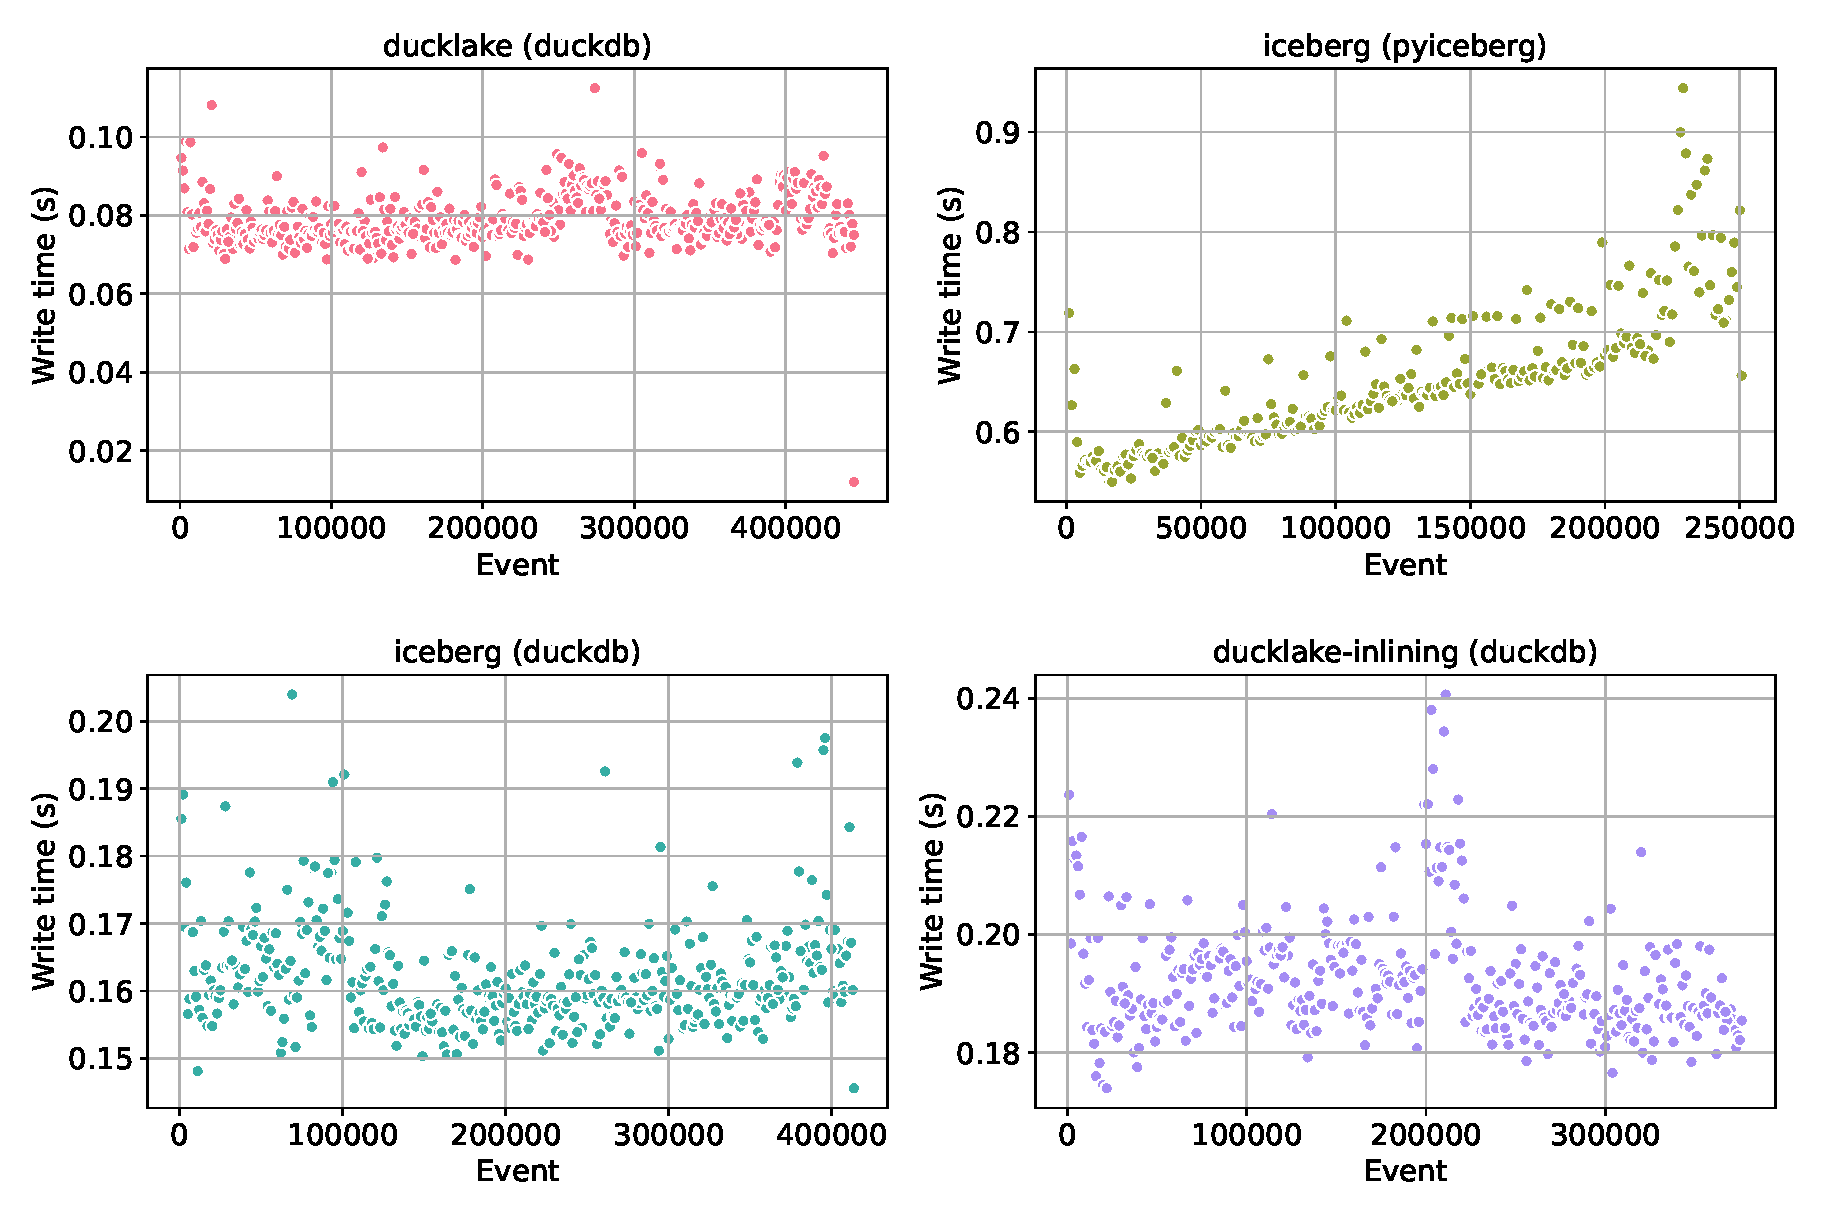
\includegraphics[width=\linewidth]{imgs/scatter-write-times-over-time-batched.eps}
	\caption{Scatter plot of time spent writing batches of 1,000 events to the lakehouse tables during the first warm run, in seconds.}
	\label{fig:scatter-write-times-over-time-batched}
\end{figure}

\subsection{Read times}
The read times of all runs (Figure \ref{fig:box-read-times-batched}) were very similar to each other, with the Q3 for all box plots being below 0.1 milliseconds. We can again confirm that no SUT had an unfair advantage caused by significantly faster read times of our benchmark tool.

\begin{figure}[h!]
	\centering
	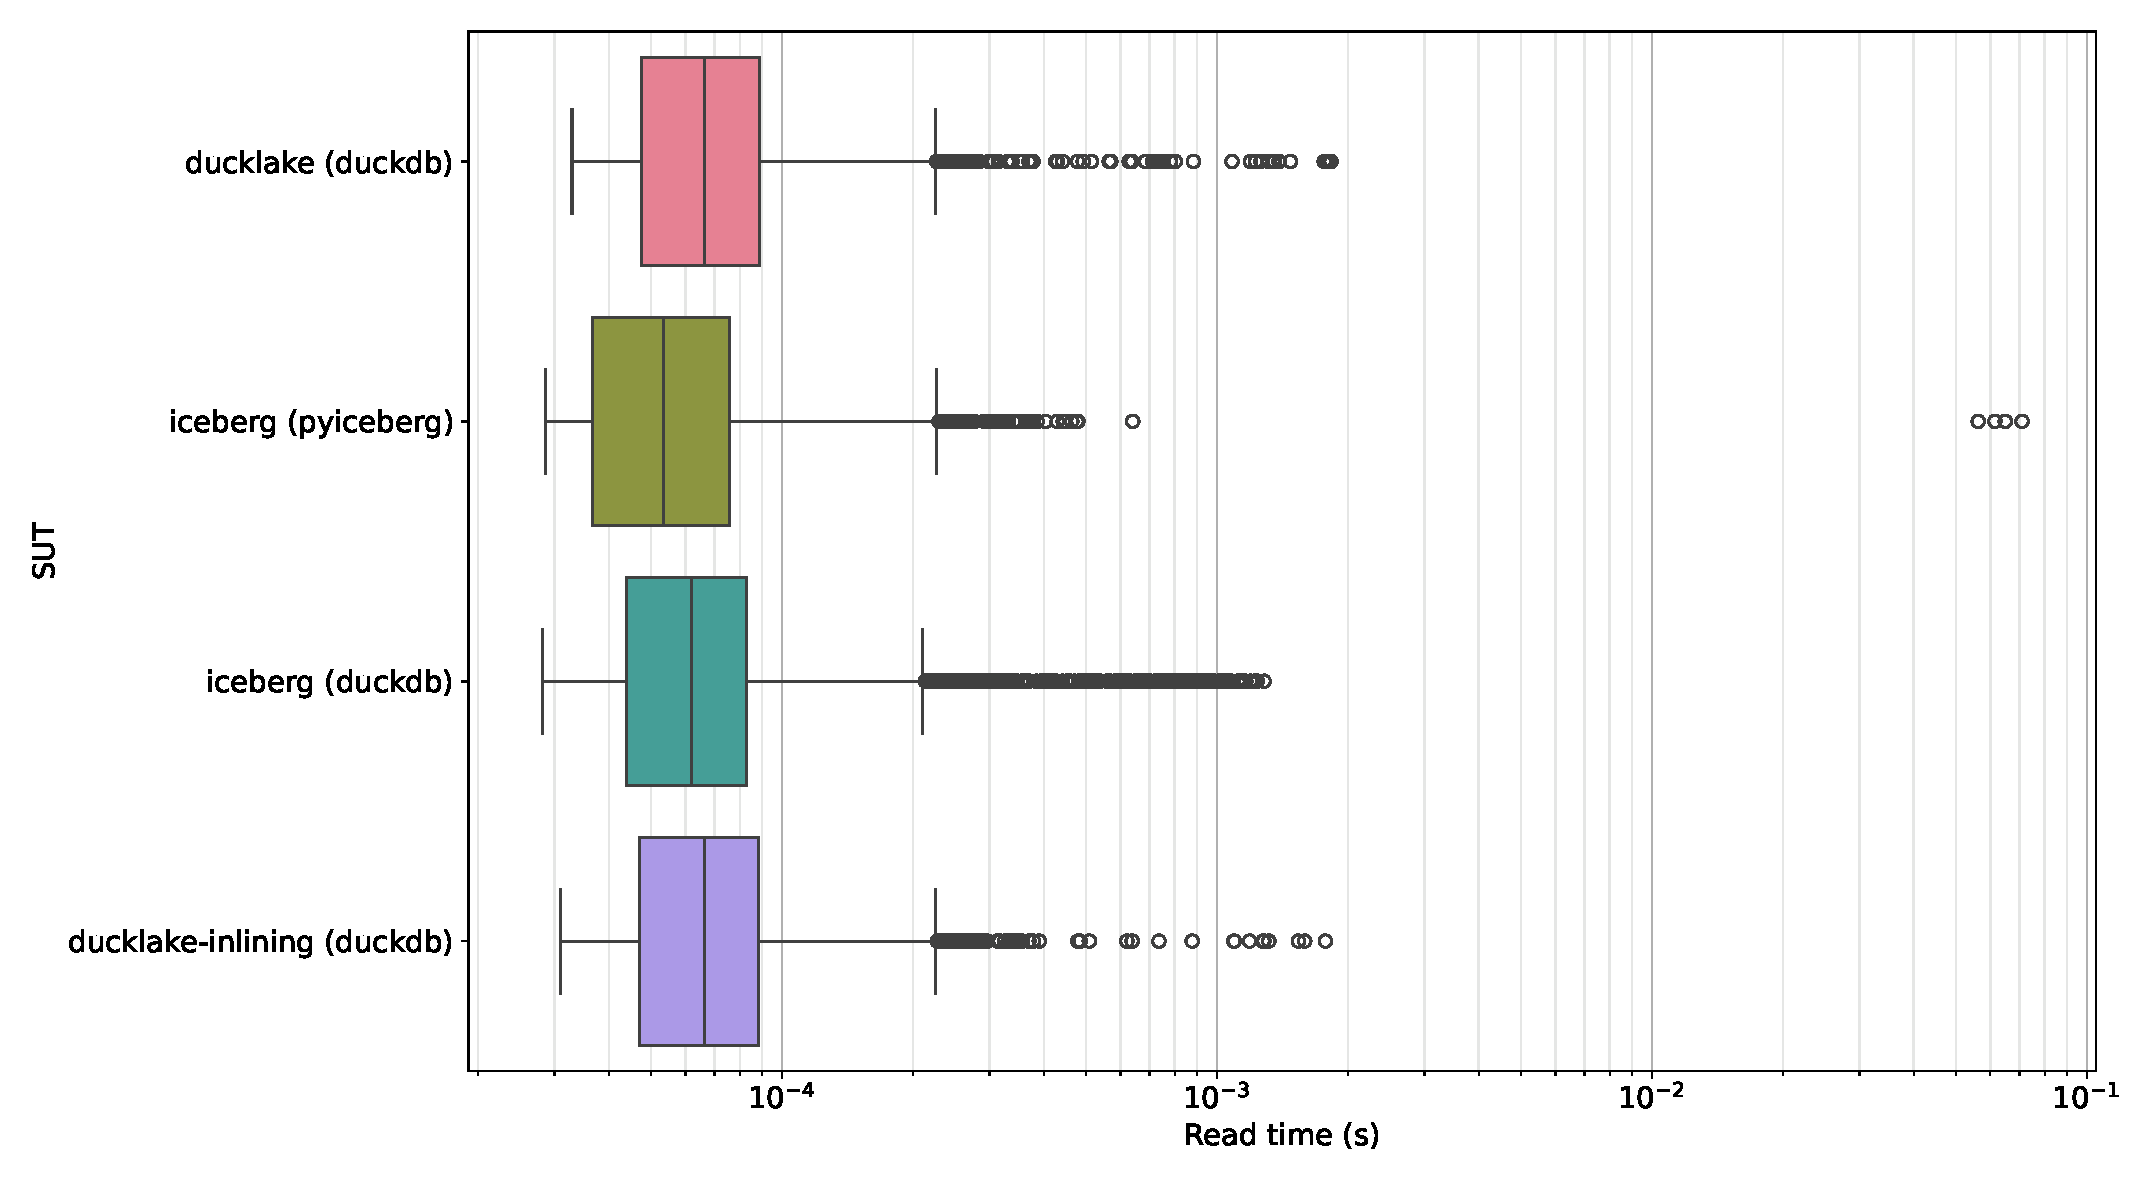
\includegraphics[width=\linewidth]{imgs/box-read-times-batched.eps}
	\caption{Box plots of the time spent reading individual events from Kafka during the first warm run of each SUT, in seconds.}
	\label{fig:box-read-times-batched}
\end{figure}

\subsection{CPU usage}
In terms of CPU usage, all systems presented very similar percentages throughout their runs, as we can see in Figure \ref{fig:cpu-usage-batched-events}. DuckLake instances showed slightly higher CPU percentages overall than Iceberg. We also see that all four runs had a dip and spike around halfway through, which is likely due to some underlying operation running in the local machine's OS.

\begin{figure}[h!]
	\centering
	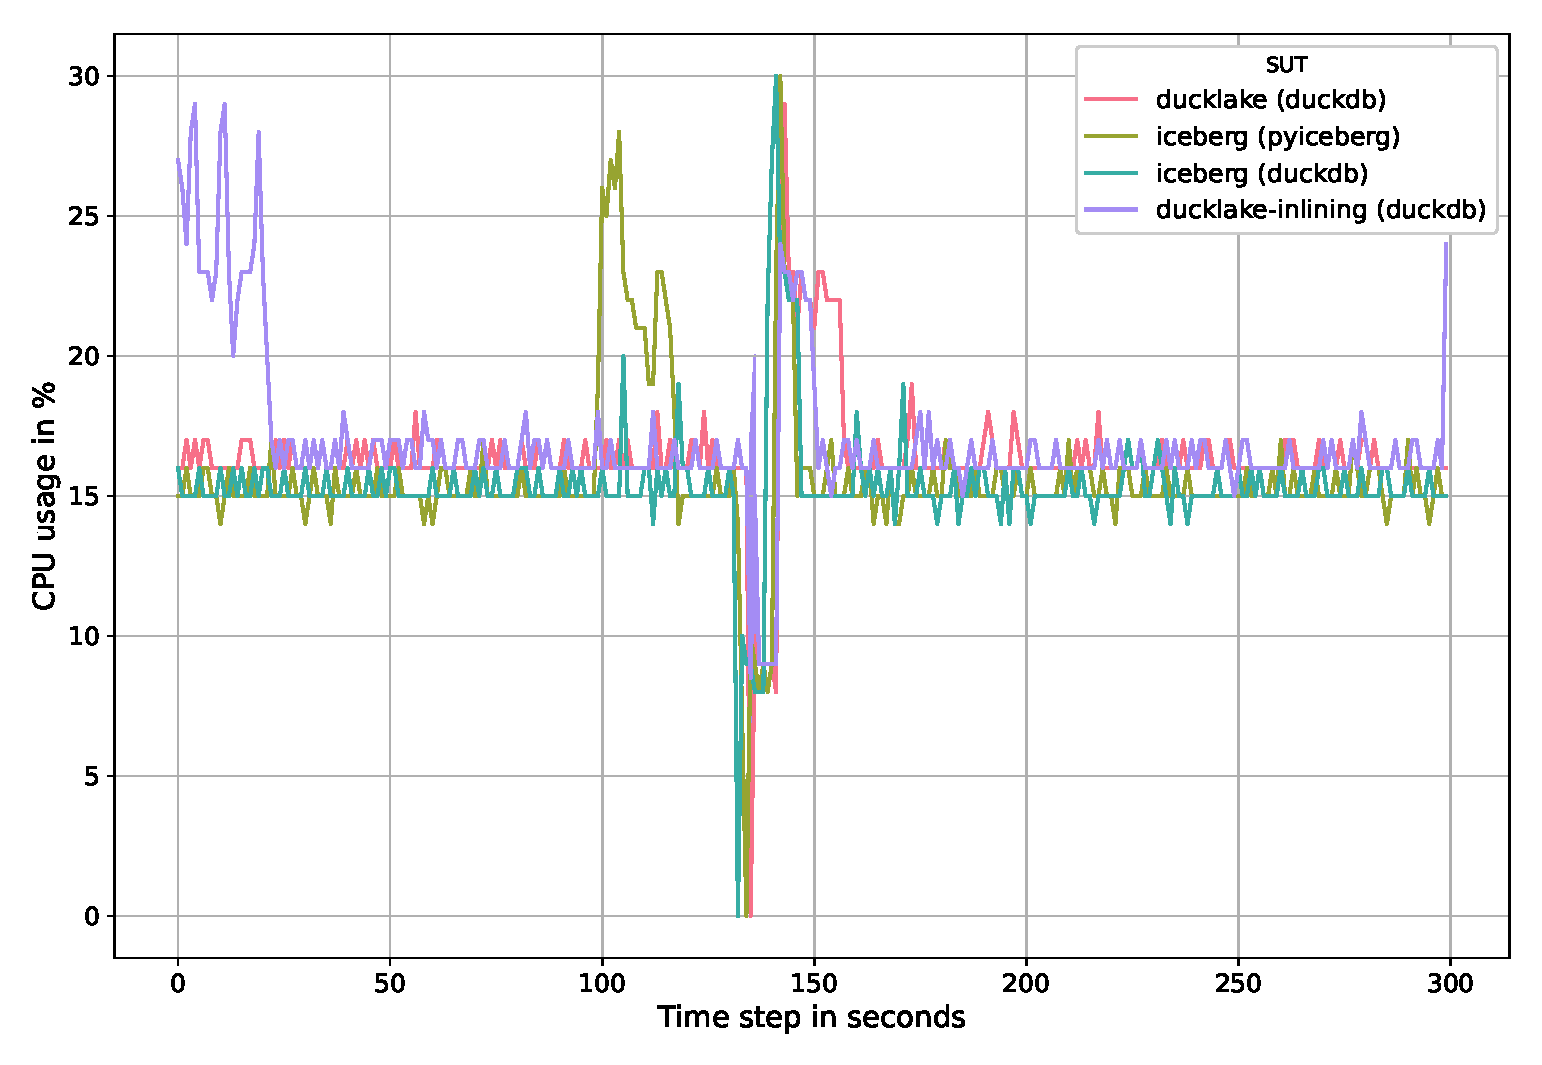
\includegraphics[width=\linewidth]{imgs/cpu-usage-batched-events.eps}
	\caption{Time spent reading individual events from Kafka during the first warm run of each SUT. The measurements were taken using time.perf\_counter\_ns.}
	\label{fig:cpu-usage-batched-events}
\end{figure}


